% SystemLimitationsAndConsiderations.tex
\section{System Limitations And Considerations}
This section discusses the limitations and future work.
\subsection{\acf{RED} testbench limitations and impact}
The Renewable Energy Demonstrator (RED) device borrowed from the EPS team \cite{RefWorks:shopov2022renewable} proved to be valuable as a testbench for our project, but several limitations affected our ability to gather comprehensive data for accurate sun vector determination.
\subsubsection{Servo Motor Limitations}
There were at least two issues with the Servo Motors which reduced our ability to gether data:
\begin{itemize}
    \item Inablity to reach the target angles requested in code without phisical intervention, presumably due to insufficient torque or gearing issues.
    \item Control deadband did not allow us to gather a large enough sample (small-angle adjustment) to create a \ac{LUT} that would allow the prediction of light position by interpolation.
\end{itemize}

When attempting to move from 0\textdegree{} to 90\textdegree{}, for example, the servomotors would often stall, requiring manual assistance to ``help'' the arch reach the desired position. This introduced inconsistency in our testing methodology and required manual adjustment using protractors.

\subsubsection{Signal Interference Issues}

The \ac{RED}'s Power Supply interference made the signal very noisy. However due to the nature of the high frequency noise and low frequency signal, it meant that it was relativly easy to filter using the scipy.signal library \cite{RefWorks:butter}, detailed in Section \ref{LowPassFilter}. Further, arch position changing without pressing the button likely due to noise in the \ac{RED} from the Power Supply made testing slighlty more annoying, but it was not happening often enough to disrupt testing too much, it was considered an acceptable quirk.

\subsubsection{Impact on Look-Up Table development}

The most significant impact to the project caused by these issues with the \ac{RED} are that we were unable to generate a \ac{LUT} or a "Sensor Response Surface" plot using the prototype, as the angle precision from the arch was not good enough. Originally, our plan included:

\begin{itemize}
    \item Taking measurements at fine angular increments (every 5\textdegree{}) across the hemisphere
    \item Mapping between sensor readings and light source position
    \item Using said mapping to develop interpolation algorithms for positions between measured points
    \item Validating position determination accuracy across the sensor's field of view
\end{itemize}

The compbination of these limitations of the \ac{RED} testbench made it impractical to gather the comprehensive dataset required to fulfill these goals, as without a reliable dataset across the entire \ac{FOV} it is not possible to predict the location of light.
These limitations ultimatly directly affected the ability to detect the light position, and we could only take some readings and compare them to the simulated environment. These comparison were ultimatly close, therefore it is believed that with better testbench accuracy, the \ac{LUT} and ability to "read" new light positions would be possible.

\subsection{Aperture placement accuracy}

Another big limitation on accuracy of the readings will be the manually placed apertures. As shown earlier in Figure \ref{fig:aperturePhoto}, the apertures are far from perfectly in the middle. This will have a huge impact on the accuracy of the readings especially when compared to a simulated environment which have perfectly placed apertures. Howver, if we had been able to create a \ac{LUT} using the real measurements with aperture as-is, the results could have theoretically been used to read the location of light. Unfortunately, as stated above, that was also impossible due to the limitations of the testbench. These two main factors were the main cause of not being able to perform a calibration and perform actual readings to test the ability to read light locations. 

\subsection{Model Limitations and Future Work}
\begin{itemize}
    \item The vertical scale differs between plots figure~\ref{fig:Model and Physical Results Comparison}: simulated hits are relative percentages, while the experimental data reflects voltage. A calibration factor could be introduced in future to improve this correspondence.
    \item Minor asymmetries in the experimental data may arise from mechanical inaccuracies or misalignment, which are not currently modelled.
    \item Future improvements may incorporate ray divergence, non-ideal optics, or sensor sensitivity profiles to further refine realism.
\end{itemize}

% Your content here

% \subsection{}
% Your content here

% \subsection{}


% Example figure jpg
%
% \begin{figure}[htb]
%     \centering
%     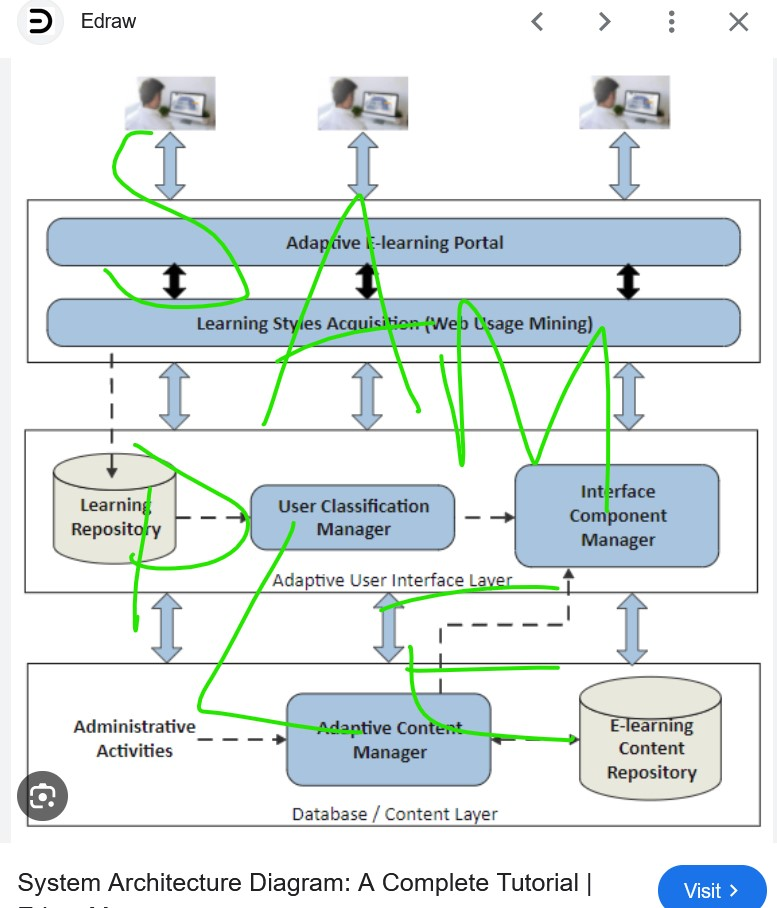
\includegraphics[width=1\textwidth]{figures/results/system_architecture.jpg}
%     \caption{Overall System Performance Analysis}
%     \label{fig:systemPerformance}
% \end{figure}

% Example listing (such as text output from console)
% \begin{figure}[H]
%     \begin{lstlisting}[style=cstyle]
%     // Environmental test results
%     // Temperature, ambient light, and vibration effects
%     \end{lstlisting}
%     \caption{Environmental Testing Results}
%     \label{lst:EnvironmentalTests1}
%     \end{figure}



% Example LATEX flowchart
% Include a flowchart
% \begin{figure}[H]
%     \centering
%     \scalebox{0.8}{ % Scale to 80% of original size
%         % try generating flowcharts as svg in Claude 
% and edit with inkscape instead of this.
% but claude did generate this one so might 
% be useful too but you can't easily make
% small repairs in inkscape


% CNN Transfer Learning Flowchart - Compact Multi-Column Layout
% \begin{figure}[htbp]

\centering
\resizebox{\textwidth}{!}{ % Scale to fit width while maintaining aspect ratio
\begin{tikzpicture}[node distance=0.8cm and 1.5cm, auto]
    % Define a smaller block style
    \tikzset{
      block/.style = {rectangle, draw, fill=blue!20, 
                      text width=7em, text centered, rounded corners, minimum height=1.8em, font=\small},
    }
    
    % Brazilian model training - Column 1
    \node [block] (brazildata) {Download Brazilian coins dataset};
    \node [block, below=of brazildata] (extract) {Extract dataset};
    \node [block, below=of extract] (setup) {Setup directories};
    \node [block, below=of setup] (define) {Define train/val dirs};
    \node [block, below=of define] (create) {Create CNN architecture};
    \node [block, below=of create] (compile) {Compile the CNN};
    \node [block, below=of compile] (train) {Train model};
    \node [block, below=of train] (trained) {Model trained (5 classes)};
    
    % Transfer learning - Column 2 (Middle)
    \node [block, right=2.5cm of brazildata] (freeze) {Freeze all layers};
    \node [block, below=of freeze] (replace) {Replace final layers};
    \node [block, below=of replace] (add) {Add regularization and dropout};
    \node [block, below=of add] (output) {New output layer (8 classes)};
    \node [block, below=of output] (finaltrain) {Train and fine-tune};
    \node [block, below=of finaltrain] (inference) {Perform inference on new coins};
    
    % UK data preparation - Column 3 (Right)
    \node [block, right=2.5cm of freeze] (ukdata) {Download UK coins dataset};
    \node [block, below=of ukdata] (ukextract) {Extract UK dataset};
    \node [block, below=of ukextract] (uksetup) {Setup UK directories};
    \node [block, below=of uksetup] (ukgen) {Create data generators (80/20 split)};
    
    % Connect all nodes with arrows
    \path [line] (brazildata) -- (extract);
    \path [line] (extract) -- (setup);
    \path [line] (setup) -- (define);
    \path [line] (define) -- (create);
    \path [line] (create) -- (compile);
    \path [line] (compile) -- (train);
    \path [line] (train) -- (trained);
    
    \path [line] (ukdata) -- (ukextract);
    \path [line] (ukextract) -- (uksetup);
    \path [line] (uksetup) -- (ukgen);
    
    % Connect the columns
    \path [line] (trained) -- node[midway, above] {Transfer} (freeze);
    \path [line] (ukgen) |- (finaltrain);
    
    % Connect middle column
    \path [line] (freeze) -- (replace);
    \path [line] (replace) -- (add);
    \path [line] (add) -- (output);
    \path [line] (output) -- (finaltrain);
    \path [line] (finaltrain) -- (inference);
    
    % Group boxes to show different stages with smaller padding
    \begin{pgfonlayer}{background}
        \node[group={[yshift=0.3cm]above:Brazilian Model Training}, fit={(brazildata) (extract) (setup) (define) (create) (compile) (train) (trained)}, inner sep=0.2cm] {};
        \node[group={[yshift=0.3cm]above:UK Data Preparation}, fit={(ukdata) (ukextract) (uksetup) (ukgen)}, inner sep=0.2cm] {};
        \node[group={[yshift=0.3cm]above:Transfer Learning}, fit={(freeze) (replace) (add) (output) (finaltrain) (inference)}, inner sep=0.2cm] {};
    \end{pgfonlayer}
\end{tikzpicture}
}
% \caption{CNN Transfer Learning Flowchart: Brazilian to UK Coins}
% \label{fig:cnn-flowchart}
% \end{figure}
%     }
%     \caption{System Design Overview Flowchart}
%     \label{fig:decriptiveLabel4} % descriptive to call in text with \ref{fig:decriptiveLabel}
% \end{figure}